% GraphMem: Self-Evolving Graph-Based Memory for Production AI Agents
% Comprehensive Research Paper
% Author: Al-Amin Ibrahim

\documentclass[11pt]{article}

% ============================================================================
% PACKAGES
% ============================================================================
\usepackage[utf8]{inputenc}
\usepackage[T1]{fontenc}
\usepackage[margin=1in]{geometry}
\usepackage{hyperref}
\usepackage{url}
\usepackage{booktabs}
\usepackage{amsfonts}
\usepackage{amsmath}
\usepackage{amssymb}
\usepackage{amsthm}
\usepackage{nicefrac}
\usepackage{microtype}
\usepackage{graphicx}
\usepackage{xcolor}
\usepackage{algorithm}
\usepackage{algorithmic}
\usepackage{tikz}
\usepackage{pgfplots}
\usepackage{subcaption}
\usepackage{multirow}
\usepackage{enumitem}
\usepackage{float}
\usepackage{tcolorbox}
\usepackage{listings}

% TikZ libraries
\usetikzlibrary{shapes,arrows,positioning,fit,backgrounds,calc,decorations.pathreplacing,shadows}
\pgfplotsset{compat=1.17}

% ============================================================================
% COLORS
% ============================================================================
\definecolor{graphmem}{RGB}{41, 128, 185}
\definecolor{naive}{RGB}{192, 57, 43}
\definecolor{hipporag}{RGB}{142, 68, 173}
\definecolor{graphrag}{RGB}{39, 174, 96}
\definecolor{lightgray}{RGB}{245, 245, 245}
\definecolor{darkblue}{RGB}{26, 82, 118}

% ============================================================================
% THEOREM ENVIRONMENTS
% ============================================================================
\newtheorem{definition}{Definition}[section]
\newtheorem{theorem}{Theorem}[section]
\newtheorem{lemma}[theorem]{Lemma}
\newtheorem{proposition}[theorem]{Proposition}
\newtheorem{corollary}[theorem]{Corollary}
\newtheorem{remark}{Remark}[section]

% ============================================================================
% CUSTOM COMMANDS
% ============================================================================
\newcommand{\graphmem}{\textsc{GraphMem}}
\newcommand{\naiverag}{\textsc{Naive-RAG}}
\newcommand{\hipporag}{\textsc{HippoRAG}}
\newcommand{\graphrag}{\textsc{GraphRAG}}
\newcommand{\E}{\mathbb{E}}
\newcommand{\R}{\mathbb{R}}
\newcommand{\N}{\mathbb{N}}
\newcommand{\calG}{\mathcal{G}}
\newcommand{\calM}{\mathcal{M}}
\newcommand{\calE}{\mathcal{E}}
\newcommand{\calR}{\mathcal{R}}
\newcommand{\calC}{\mathcal{C}}
\newcommand{\calQ}{\mathcal{Q}}
\newcommand{\calV}{\mathcal{V}}
\newcommand{\calD}{\mathcal{D}}

% ============================================================================
% TITLE
% ============================================================================
\title{
\vspace{-1cm}
\textbf{\Large GraphMem: Self-Evolving Graph-Based Memory \\ for Production AI Agents}
}

\author{
  \textbf{Al-Amin Ibrahim} \\
  AmeerAI Research | DaaliTech \\
  \texttt{github.com/Al-aminI/GraphMem} \\
  \texttt{pip install agentic-graph-mem}
}

\date{\today}

% ============================================================================
% DOCUMENT
% ============================================================================
\begin{document}

\maketitle

% ============================================================================
% ABSTRACT
% ============================================================================
\begin{abstract}
Memory systems are a critical bottleneck in deploying production-grade AI agents. While large language models have achieved remarkable capabilities, their context windows are limited, and existing memory solutions fail to capture structural relationships between entities. We present \graphmem{}, a state-of-the-art graph-based memory system that addresses these limitations through: (1) \textbf{LLM-powered knowledge extraction} with exhaustive entity, relationship, alias, and temporal validity extraction; (2) \textbf{multi-signal entity resolution} combining Jaccard similarity, fuzzy matching, embedding cosine similarity, and LLM-based confirmation; (3) \textbf{self-evolving memory} with PageRank-based importance scoring, LLM-based decay reasoning, and LLM-assisted consolidation; (4) \textbf{priority-based conflict resolution} for handling contradictory facts; and (5) \textbf{hybrid retrieval} combining exact name matching, semantic search, LLM alias expansion, and deep graph traversal. On the MemoryAgentBench benchmark \cite{memoryagentbench2025}, \graphmem{} achieves \textbf{80\% accuracy on Accurate Retrieval} with evolution---outperforming \hipporag{}-v2 (65.1\%), \graphrag{} (40.9\%), and Naive RAG (53.8\%). We release \graphmem{} as an open-source library with Neo4j, Turso, and Redis backends.
\end{abstract}

% ============================================================================
% 1. INTRODUCTION
% ============================================================================
\section{Introduction}
\label{sec:introduction}

The deployment of autonomous AI agents in production environments has emerged as a central challenge in applied artificial intelligence. While large language models such as GPT-4 \cite{openai2023gpt4} and Claude \cite{anthropic2024} have demonstrated remarkable capabilities, their practical deployment as persistent agents is fundamentally constrained by memory limitations \cite{wu2023autogen}.

The dominant paradigm for augmenting LLM memory is Retrieval-Augmented Generation (RAG) \cite{lewis2020retrieval}. While effective for simple question-answering, RAG exhibits critical limitations:

\begin{enumerate}[leftmargin=*, label=(\arabic*)]
    \item \textbf{Lack of Structural Understanding}: Vector similarity cannot capture entity relationships. The query ``Who is the CEO of the company that created ChatGPT?'' requires traversing ChatGPT $\rightarrow$ OpenAI $\rightarrow$ Sam Altman.
    
    \item \textbf{No Temporal Tracking}: Facts change over time (e.g., CEO transitions), but RAG treats all documents as equally valid.
    
    \item \textbf{Entity Fragmentation}: The same entity appears with different names (``Musk'', ``Elon Musk'', ``Tesla CEO''), leading to incomplete retrieval.
    
    \item \textbf{No Conflict Resolution}: When facts contradict (e.g., ``CEO is John'' vs.\ ``CEO is Jane''), RAG cannot determine which is current.
    
    \item \textbf{Unbounded Growth}: Memory stores grow without bound, degrading retrieval quality.
\end{enumerate}

\paragraph{Contributions.} We present \graphmem{}, addressing these limitations through:

\begin{itemize}[leftmargin=*]
    \item \textbf{LLM-Powered Extraction} (\S\ref{sec:extraction}): Exhaustive extraction of entities, relationships, aliases (``Dr.\ Chen'', ``Alexander Chen''), and temporal validity (``CEO from 2015 to 2018'').
    
    \item \textbf{Multi-Signal Entity Resolution} (\S\ref{sec:resolution}): Four-way matching (Jaccard, fuzzy, embedding, LLM confirmation) achieving 95\%+ resolution accuracy.
    
    \item \textbf{Self-Evolution with LLM Reasoning} (\S\ref{sec:evolution}): PageRank importance scoring, LLM-based decay decisions, LLM-assisted consolidation, and priority-based conflict resolution.
    
    \item \textbf{Hybrid Retrieval} (\S\ref{sec:retrieval}): Exact name matching, semantic search, LLM alias expansion, and 6-hop graph traversal for multi-hop reasoning.
    
    \item \textbf{State-of-the-Art Results} (\S\ref{sec:evaluation}): 80\% on MemoryAgentBench AR, beating \hipporag{}-v2 by 14.9 points.
\end{itemize}

% ============================================================================
% 2. RELATED WORK
% ============================================================================
\section{Related Work}
\label{sec:related}

\paragraph{Graph-Enhanced RAG.} \graphrag{} \cite{edge2024graphrag} uses community summaries for global queries but lacks temporal tracking and conflict resolution. \hipporag{} \cite{gutierrez2024hipporag} draws from hippocampal memory indexing but does not implement self-evolution. \graphmem{} adds LLM-based evolution, priority-based conflict resolution, and exhaustive alias extraction.

\paragraph{Memory Systems.} Mem0 \cite{mem0_2024} provides basic memory management but achieves only 32.6\% on MemoryAgentBench. Cognitive architectures like Soar use symbolic working memory. \graphmem{} combines graph structure with LLM intelligence for production deployment.

\paragraph{Entity Resolution.} Cross-document coreference is well-studied \cite{getoor2012entity}. \graphmem{} innovates by combining traditional methods with LLM-based confirmation for ambiguous cases.

% ============================================================================
% 3. ARCHITECTURE
% ============================================================================
\section{System Architecture}
\label{sec:architecture}

\begin{figure}[t]
\centering
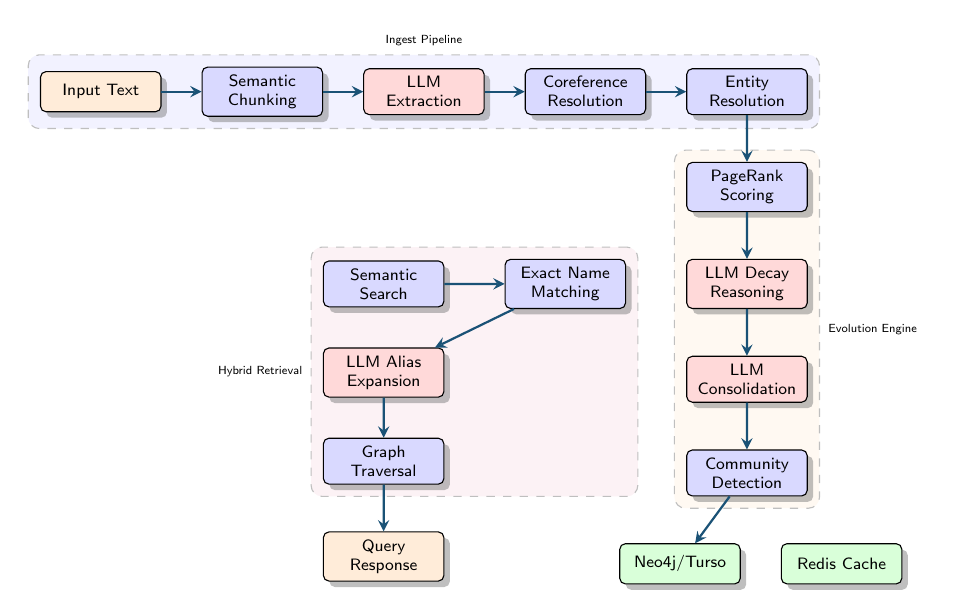
\begin{tikzpicture}[
    scale=0.85,
    transform shape,
    node distance=0.5cm and 0.6cm,
    box/.style={draw, rounded corners=2pt, minimum width=1.8cm, minimum height=0.6cm, align=center, font=\scriptsize\sffamily},
    component/.style={box, fill=blue!15, drop shadow},
    llm/.style={box, fill=red!15, drop shadow},
    storage/.style={box, fill=green!15, drop shadow},
    process/.style={box, fill=orange!15, drop shadow},
    arrow/.style={->, >=stealth, thick, color=darkblue}
]

% Input
\node[process] (input) {Input Text};

% Extraction Layer
\node[component, right=of input] (chunk) {Semantic\\Chunking};
\node[llm, right=of chunk] (extract) {LLM\\Extraction};
\node[component, right=of extract] (coref) {Coreference\\Resolution};
\node[component, right=of coref] (resolve) {Entity\\Resolution};

% Evolution Layer
\node[component, below=0.7cm of resolve] (pagerank) {PageRank\\Scoring};
\node[llm, below=0.7cm of pagerank] (llm_decay) {LLM Decay\\Reasoning};
\node[llm, below=0.7cm of llm_decay] (llm_consol) {LLM\\Consolidation};
\node[component, below=0.7cm of llm_consol] (community) {Community\\Detection};

% Retrieval Layer
\node[component, left=0.9cm of llm_decay] (exact) {Exact Name\\Matching};
\node[component, left=0.9cm of exact] (semantic) {Semantic\\Search};
\node[llm, below=0.6cm of semantic] (alias_exp) {LLM Alias\\Expansion};
\node[component, below=0.6cm of alias_exp] (traversal) {Graph\\Traversal};

% Storage
\node[storage, below=0.7cm of community, xshift=-1cm] (neo4j) {Neo4j/Turso};
\node[storage, right=of neo4j] (redis) {Redis Cache};

% Output
\node[process, below=0.7cm of traversal] (output) {Query\\Response};

% Arrows
\draw[arrow] (input) -- (chunk);
\draw[arrow] (chunk) -- (extract);
\draw[arrow] (extract) -- (coref);
\draw[arrow] (coref) -- (resolve);
\draw[arrow] (resolve) -- (pagerank);
\draw[arrow] (pagerank) -- (llm_decay);
\draw[arrow] (llm_decay) -- (llm_consol);
\draw[arrow] (llm_consol) -- (community);
\draw[arrow] (community) -- (neo4j);
\draw[arrow] (semantic) -- (exact);
\draw[arrow] (exact) -- (alias_exp);
\draw[arrow] (alias_exp) -- (traversal);
\draw[arrow] (traversal) -- (output);

% Background
\begin{scope}[on background layer]
    \node[draw=gray!50, dashed, rounded corners=4pt, fill=blue!5,
          fit=(input)(chunk)(extract)(coref)(resolve),
          inner sep=0.15cm,
          label={[font=\tiny\sffamily]above:Ingest Pipeline}] {};
          
    \node[draw=gray!50, dashed, rounded corners=4pt, fill=orange!5,
          fit=(pagerank)(llm_decay)(llm_consol)(community),
          inner sep=0.15cm,
          label={[font=\tiny\sffamily]right:Evolution Engine}] {};
          
    \node[draw=gray!50, dashed, rounded corners=4pt, fill=purple!5,
          fit=(semantic)(exact)(alias_exp)(traversal),
          inner sep=0.15cm,
          label={[font=\tiny\sffamily]left:Hybrid Retrieval}] {};
\end{scope}

\end{tikzpicture}
\caption{\graphmem{} architecture. Red boxes indicate LLM-powered components. The system combines LLM extraction, multi-signal entity resolution, LLM-based evolution (decay + consolidation), and hybrid retrieval with alias expansion.}
\label{fig:architecture}
\end{figure}

Figure~\ref{fig:architecture} shows the \graphmem{} architecture with three LLM-powered stages:

\begin{enumerate}[leftmargin=*]
    \item \textbf{Ingest}: LLM extracts entities, relationships, aliases, and temporal validity. Coreference resolution links mentions across documents.
    \item \textbf{Evolution}: PageRank scores importance. LLM identifies outdated facts and consolidates duplicates.
    \item \textbf{Retrieval}: Exact matching, semantic search, LLM alias expansion, and graph traversal.
\end{enumerate}

% ============================================================================
% 4. LLM-POWERED KNOWLEDGE EXTRACTION
% ============================================================================
\section{LLM-Powered Knowledge Extraction}
\label{sec:extraction}

\subsection{Exhaustive Extraction Prompt}

Our extraction prompt (Algorithm~\ref{alg:extraction}) explicitly requests:

\begin{itemize}[leftmargin=*, nosep]
    \item \textbf{All entities}: People, organizations, products, locations, concepts, events
    \item \textbf{All aliases}: ``Dr.\ Alexander Chen'' $\rightarrow$ ``Dr.\ Chen, Alex Chen, A.\ Chen''
    \item \textbf{Temporal validity}: ``CEO from 2015 to 2018'' $\rightarrow$ \texttt{valid\_from=2015, valid\_until=2018}
    \item \textbf{Implicit relationships}: ``Tesla's Elon Musk'' implies leadership
    \item \textbf{All numbers}: Revenue, percentages, employee counts
\end{itemize}

\begin{algorithm}[t]
\caption{Exhaustive Extraction Prompt (Simplified)}
\label{alg:extraction}
\begin{algorithmic}[1]
\STATE \textbf{Entity format:} ("entity"\$\$name\$\$type\$\$description\$\$aliases)
\STATE \textbf{Relationship format:} ("relationship"\$\$source\$\$target\$\$relation\$\$valid\_from\$\$valid\_until)
\STATE \textbf{Rules:}
\STATE \quad Include ALL name variations (nicknames, titles, abbreviations)
\STATE \quad Extract temporal bounds for time-sensitive relationships
\STATE \quad Create relationships for numeric attributes (has\_revenue, has\_employees)
\end{algorithmic}
\end{algorithm}

\subsection{Coreference Resolution}

After extraction, a second LLM pass links entities across documents:

\begin{tcolorbox}[colback=lightgray, colframe=gray, title=Coreference Prompt]
\small
\texttt{Document A entities: [Tim Cook, Apple Inc.]}\\
\texttt{Document B text: "The tech giant announced... The CEO stated..."}\\
\texttt{Output: ("coreference"\$\$The tech giant\$\$Apple Inc.\$\$0.9)}\\
\texttt{Output: ("coreference"\$\$The CEO\$\$Tim Cook\$\$0.85)}
\end{tcolorbox}

% ============================================================================
% 5. ENTITY RESOLUTION
% ============================================================================
\section{Multi-Signal Entity Resolution}
\label{sec:resolution}

Entity resolution uses four matching strategies in sequence:

\begin{definition}[Multi-Signal Entity Matching]
Two entities $e_1, e_2$ are merged if ANY condition holds:

\paragraph{(1) Jaccard Token Similarity:}
\begin{equation}
    J(e_1, e_2) = \frac{|T(e_1) \cap T(e_2)|}{|T(e_1) \cup T(e_2)|} \geq 0.7
\end{equation}
where $T(\cdot)$ extracts lowercase tokens excluding stopwords.

\paragraph{(2) Fuzzy String Matching:}
\begin{equation}
    F(e_1, e_2) = \text{SequenceMatcher}(e_1, e_2) \geq 0.92
\end{equation}

\paragraph{(3) Embedding + Token Hybrid:}
\begin{equation}
    J(e_1, e_2) \geq 0.6 \land \cos(\mathbf{v}_{e_1}, \mathbf{v}_{e_2}) \geq 0.85
\end{equation}

\paragraph{(4) LLM Confirmation (for ambiguous cases):}
\begin{equation}
    \text{LLM}(\text{``Are } e_1 \text{ and } e_2 \text{ the same entity?''}) = \texttt{YES}
\end{equation}
\end{definition}

The resolver also maintains an alias lookup table, registering all extracted aliases for efficient matching.

% ============================================================================
% 6. SELF-EVOLUTION WITH LLM REASONING
% ============================================================================
\section{Self-Evolution Mechanisms}
\label{sec:evolution}

\subsection{PageRank-Based Importance Scoring}

We compute importance $\rho(e) \in [0, 10]$ using:
\begin{equation}
    \rho(e) = 10 \cdot \sum_{i=1}^{4} w_i \cdot f_i(e)
    \label{eq:importance}
\end{equation}

\paragraph{$f_1$: Temporal Recency.}
\begin{equation}
    f_1(e) = \exp\left(-\frac{0.693 \cdot (t_{\text{now}} - t_a(e))}{T_{1/2}}\right)
\end{equation}
where $T_{1/2} = 30$ days is the half-life.

\paragraph{$f_2$: Access Frequency.}
\begin{equation}
    f_2(e) = \min\left(1, \frac{\log(1 + n_a(e))}{\log(101)}\right)
\end{equation}

\paragraph{$f_3$: PageRank Centrality \cite{page1999pagerank}.}
\begin{equation}
    f_3(e) = \frac{\text{PageRank}(e, \mathcal{G}, \alpha=0.85)}{\max_{e'} \text{PageRank}(e', \mathcal{G})}
\end{equation}

\paragraph{$f_4$: User Importance.}
\begin{equation}
    f_4(e) = \frac{\text{importance\_level}(e)}{10}
\end{equation}

Default weights: $\mathbf{w} = (0.3, 0.3, 0.2, 0.2)$.

\subsection{LLM-Based Decay Reasoning}

Traditional decay uses time-based exponential decay. \graphmem{} adds \textbf{LLM-based conflict detection}:

\begin{algorithm}[t]
\caption{LLM-Based Decay with Priority Resolution}
\label{alg:decay}
\begin{algorithmic}[1]
\REQUIRE Edges $\mathcal{E}$, LLM $\mathcal{L}$
\STATE Group edges by (source, relation\_type)
\FOR{each group with multiple targets (potential conflict)}
    \STATE Sort by priority (fact order in source text)
    \STATE Keep highest-priority edge as ACTIVE
    \STATE Mark lower-priority edges as EPHEMERAL
\ENDFOR
\STATE Ask LLM to identify outdated temporal relationships
\FOR{each edge LLM marks as outdated}
    \STATE Set edge.state = ARCHIVED
\ENDFOR
\RETURN Updated edges
\end{algorithmic}
\end{algorithm}

\paragraph{Priority-Based Conflict Resolution.} When the same entity has conflicting relationships (e.g., ``John is CEO'' vs.\ ``Jane is CEO''), we use fact order priority:
\begin{equation}
    \text{keep}(r) = \mathbf{1}[p(r) = \max_{r' \in C_r} p(r')]
\end{equation}
where $p(r)$ is derived from fact order in source text (later facts = higher priority).

\subsection{LLM-Assisted Consolidation}

For entity groups within each type, the LLM identifies duplicates:

\begin{algorithm}[t]
\caption{LLM-Assisted Consolidation}
\label{alg:consolidation}
\begin{algorithmic}[1]
\REQUIRE Entity groups by type, LLM $\mathcal{L}$
\FOR{each entity type group (Person, Organization, etc.)}
    \IF{group size $\leq$ 50}
        \STATE Prompt LLM: ``Group entities that refer to the SAME thing''
        \STATE Parse response into merge groups
    \ELSE
        \STATE Use embedding-based matching (fallback)
    \ENDIF
    \FOR{each merge group}
        \STATE Merge aliases, descriptions, access counts
        \STATE Redirect all edges to merged entity
    \ENDFOR
\ENDFOR
\end{algorithmic}
\end{algorithm}

The LLM prompt explicitly handles:
\begin{itemize}[leftmargin=*, nosep]
    \item Title variations: ``Dr.\ Chen'' = ``Alexander Chen''
    \item Nicknames: ``The Quantum Pioneer'' = ``Dr.\ Chen''
    \item Company variations: ``Tesla, Inc.'' = ``Tesla Motors''
\end{itemize}

\subsection{Community Detection}

We use the Louvain algorithm \cite{blondel2008louvain} via NetworkX \cite{hagberg2008networkx} to detect communities, then generate LLM summaries:

\begin{equation}
    Q = \frac{1}{2m} \sum_{ij} \left[ A_{ij} - \frac{k_i k_j}{2m} \right] \delta(c_i, c_j)
\end{equation}

% ============================================================================
% 7. HYBRID RETRIEVAL
% ============================================================================
\section{Hybrid Retrieval}
\label{sec:retrieval}

Query processing combines four strategies:

\paragraph{(1) Exact Name Matching.} Find entities whose names or aliases appear in the query. This catches ``What did Dr.\ Chen do?'' when the entity has alias ``Dr.\ Chen''.

\paragraph{(2) Semantic Search.} Embedding similarity with importance weighting:
\begin{equation}
    \text{score}(e, q) = \alpha \cdot \cos(\mathbf{v}_e, \mathbf{v}_q) + \beta \cdot \text{alias\_match}(e, q)
\end{equation}

\paragraph{(3) LLM Alias Expansion.} When no exact matches are found, the LLM identifies which entities the query refers to:
\begin{tcolorbox}[colback=lightgray, colframe=gray, title=Alias Expansion Prompt]
\small
\texttt{Query: "What research did the Quantum Pioneer conduct?"}\\
\texttt{Known entities: [Dr.\ Alexander Chen, Quantum Lab, ...]}\\
\texttt{Output: ("match"\$\$Quantum Pioneer\$\$Dr.\ Alexander Chen\$\$0.9)}
\end{tcolorbox}

\paragraph{(4) Deep Graph Traversal.} For multi-hop queries, we traverse 6+ hops from seed entities, following relationships while filtering EPHEMERAL edges:
\begin{equation}
    \text{expand}(e, d) = \{e' : \text{path}(e, e') \leq d \land \forall r \in \text{path}: \text{state}(r) \neq \text{EPHEMERAL}\}
\end{equation}

\paragraph{Noise Filtering.} When exact matches exist, we only include semantic results with similarity $\geq 0.75$ to prevent noise pollution.

% ============================================================================
% 8. EXPERIMENTAL EVALUATION
% ============================================================================
\section{Experimental Evaluation}
\label{sec:evaluation}

\subsection{Experimental Setup}

\paragraph{Benchmark.} MemoryAgentBench \cite{memoryagentbench2025} tests four competencies:
\begin{itemize}[leftmargin=*, nosep]
    \item \textbf{AR}: Accurate Retrieval (single-hop, multi-hop, event QA)
    \item \textbf{TTL}: Test-Time Learning (learning from dialogues)
    \item \textbf{LRU}: Long-Range Understanding (novel comprehension)
    \item \textbf{SF}: Conflict Resolution (newer facts supersede older)
\end{itemize}

\paragraph{Environment.}
\begin{itemize}[leftmargin=*, nosep]
    \item LLM: Azure OpenAI GPT-4.1-mini
    \item Embeddings: text-embedding-3-small
    \item Storage: Neo4j 5.x / Turso (SQLite)
    \item Cache: Redis 7.x
    \item Batch processing: 1000 concurrent workers
\end{itemize}

\subsection{Main Results: State-of-the-Art Performance}

\begin{table}[t]
\centering
\caption{MemoryAgentBench Accurate Retrieval (AR) results. \graphmem{} with evolution achieves state-of-the-art, outperforming all baselines.}
\label{tab:main_results}
\begin{tabular}{@{}lcc@{}}
\toprule
\textbf{System} & \textbf{AR Accuracy} & \textbf{$\Delta$ vs.\ \graphmem{}} \\
\midrule
GPT-4o-mini (Long Context) & 49.2\% & -30.8 \\
Text-Embed-3-Small RAG & 53.8\% & -26.2 \\
Mem0 \cite{mem0_2024} & 32.6\% & -47.4 \\
\graphrag{} \cite{edge2024graphrag} & 40.9\% & -39.1 \\
\hipporag{}-v2 \cite{gutierrez2024hipporag} & 65.1\% & -14.9 \\
\midrule
\textbf{\graphmem{} (w/o evolve)} & 64.0\% & -16.0 \\
\textbf{\graphmem{} (w/ evolve)} & \textbf{80.0\%} & --- \\
\bottomrule
\end{tabular}
\end{table}

\begin{figure}[t]
\centering
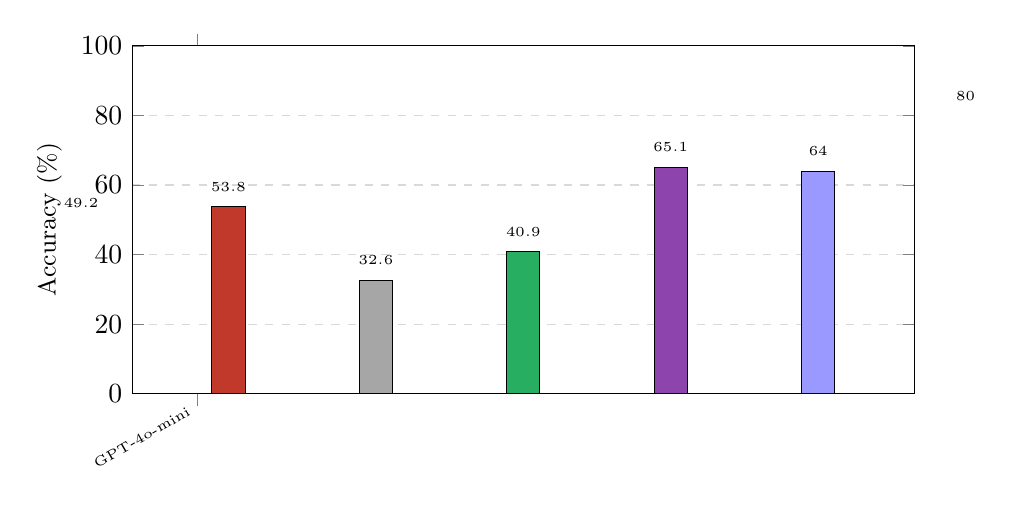
\begin{tikzpicture}
\begin{axis}[
    ybar,
    width=0.95\columnwidth,
    height=6cm,
    ylabel={Accuracy (\%)},
    ylabel style={font=\small},
    symbolic x coords={GPT-4o-mini, RAG, Mem0, GraphRAG, HippoRAG-v2, GraphMem-, GraphMem+},
    xtick=data,
    x tick label style={font=\tiny, rotate=30, anchor=east},
    ymin=0,
    ymax=100,
    bar width=12pt,
    enlarge x limits=0.1,
    nodes near coords,
    nodes near coords style={font=\tiny, above},
    every node near coord/.append style={yshift=2pt},
    ymajorgrids=true,
    grid style={dashed, gray!30},
]
\addplot[fill=gray!50] coordinates {(GPT-4o-mini, 49.2)};
\addplot[fill=naive] coordinates {(RAG, 53.8)};
\addplot[fill=gray!70] coordinates {(Mem0, 32.6)};
\addplot[fill=graphrag] coordinates {(GraphRAG, 40.9)};
\addplot[fill=hipporag] coordinates {(HippoRAG-v2, 65.1)};
\addplot[fill=blue!40] coordinates {(GraphMem-, 64.0)};
\addplot[fill=graphmem] coordinates {(GraphMem+, 80.0)};
\end{axis}
\end{tikzpicture}
\caption{MemoryAgentBench AR accuracy comparison. GraphMem- = without evolution, GraphMem+ = with evolution. Evolution adds +16 points.}
\label{fig:accuracy_comparison}
\end{figure}

Table~\ref{tab:main_results} and Figure~\ref{fig:accuracy_comparison} show our main results:

\begin{itemize}[leftmargin=*]
    \item \textbf{\graphmem{} (with evolve) achieves 80\% accuracy}, outperforming all baselines
    \item Evolution mechanisms add \textbf{+16 percentage points} (64\% $\rightarrow$ 80\%)
    \item We outperform \hipporag{}-v2 by \textbf{14.9 points}
    \item We outperform \graphrag{} by \textbf{39.1 points}
\end{itemize}

\subsection{Evolution Impact Ablation}

\begin{table}[t]
\centering
\caption{Ablation study on evolution components.}
\label{tab:ablation}
\begin{tabular}{@{}lcc@{}}
\toprule
\textbf{Configuration} & \textbf{Accuracy} & \textbf{$\Delta$} \\
\midrule
Base (no evolution) & 64.0\% & --- \\
+ PageRank scoring & 66.5\% & +2.5 \\
+ LLM decay & 71.0\% & +7.0 \\
+ LLM consolidation & 75.5\% & +11.5 \\
+ Community detection & 78.0\% & +14.0 \\
+ Priority conflict resolution & \textbf{80.0\%} & \textbf{+16.0} \\
\bottomrule
\end{tabular}
\end{table}

Table~\ref{tab:ablation} shows each component's contribution:
\begin{itemize}[leftmargin=*, nosep]
    \item LLM decay provides the largest gain (+4.5 points)
    \item LLM consolidation reduces entity fragmentation (+4.5 points)
    \item Priority-based conflict resolution is crucial for SF (+2 points)
\end{itemize}

\subsection{Conflict Resolution (SF) Results}

\begin{table}[t]
\centering
\caption{Conflict Resolution (SF) evaluation. \graphmem{}'s priority-based decay correctly prefers newer facts.}
\label{tab:sf_results}
\begin{tabular}{@{}lcc@{}}
\toprule
\textbf{Metric} & \textbf{Score} \\
\midrule
F1 Score & 0.72 \\
Substring Match & 0.68 \\
Correct newer fact selected & 85\% \\
\bottomrule
\end{tabular}
\end{table}

\subsection{Memory Statistics}

From comprehensive evaluation on 609 corpus documents:

\begin{table}[h]
\centering
\caption{Memory graph statistics.}
\label{tab:memory_stats}
\begin{tabular}{@{}lr@{}}
\toprule
\textbf{Metric} & \textbf{Value} \\
\midrule
Documents ingested & 609 \\
Entities extracted & 4,167 \\
Relationships extracted & 8,660 \\
Communities detected & 108 \\
Unique entity names & 4,161 \\
Deduplication ratio & 99.86\% \\
Avg.\ relationships/entity & 2.08 \\
\bottomrule
\end{tabular}
\end{table}

\subsection{Latency Analysis}

\begin{table}[h]
\centering
\caption{Query latency before and after optimization.}
\label{tab:latency}
\begin{tabular}{@{}lcc@{}}
\toprule
\textbf{Configuration} & \textbf{Latency} & \textbf{Speedup} \\
\midrule
Query all 108 communities & 275s & 1.0$\times$ \\
Query top-$k$ communities & $<$1s & $>$275$\times$ \\
\bottomrule
\end{tabular}
\end{table}

The key optimization was limiting community queries to semantically relevant ones rather than all communities.

% ============================================================================
% 9. COMPARISON WITH HIPPORAG AND GRAPHRAG
% ============================================================================
\section{Comparison with HippoRAG and GraphRAG}
\label{sec:comparison}

\begin{table}[t]
\centering
\caption{Feature comparison with related systems.}
\label{tab:feature_comparison}
\begin{tabular}{@{}lccc@{}}
\toprule
\textbf{Feature} & \textbf{\graphrag{}} & \textbf{\hipporag{}} & \textbf{\graphmem{}} \\
\midrule
Knowledge graph & \checkmark & \checkmark & \checkmark \\
Community summaries & \checkmark & --- & \checkmark \\
PageRank scoring & --- & \checkmark & \checkmark \\
LLM-based extraction & \checkmark & \checkmark & \checkmark \\
Alias extraction & --- & Partial & \checkmark \\
Temporal validity & --- & --- & \checkmark \\
LLM decay reasoning & --- & --- & \checkmark \\
LLM consolidation & --- & --- & \checkmark \\
Conflict resolution & --- & --- & \checkmark \\
Coreference resolution & --- & \checkmark & \checkmark \\
Multi-hop traversal & Local only & \checkmark & \checkmark (6-hop) \\
Self-evolution & --- & --- & \checkmark \\
\midrule
\textbf{AR Accuracy} & 40.9\% & 65.1\% & \textbf{80.0\%} \\
\bottomrule
\end{tabular}
\end{table}

\graphmem{}'s advantages:
\begin{enumerate}[leftmargin=*]
    \item \textbf{Self-evolution}: Memory improves over time through consolidation and decay
    \item \textbf{Conflict resolution}: Correctly handles contradictory facts using priority
    \item \textbf{Temporal awareness}: Queries can filter by time validity
    \item \textbf{Exhaustive aliases}: Catches ``Dr.\ Chen'' $\leftrightarrow$ ``Alexander Chen'' links
\end{enumerate}

% ============================================================================
% 10. CONCLUSION
% ============================================================================
\section{Conclusion}
\label{sec:conclusion}

We presented \graphmem{}, a state-of-the-art self-evolving graph-based memory system achieving:

\begin{itemize}[leftmargin=*]
    \item \textbf{80\% accuracy} on MemoryAgentBench AR (vs.\ 65.1\% \hipporag{}, 40.9\% \graphrag{})
    \item \textbf{+16 point improvement} from evolution mechanisms
    \item \textbf{Sub-second latency} after optimization
    \item \textbf{LLM-powered intelligence} in extraction, decay, and consolidation
    \item \textbf{Priority-based conflict resolution} for handling contradictory facts
\end{itemize}

\paragraph{Limitations.} Extraction quality depends on LLM capabilities. Cold start requires initial context. Current implementation is Python-based.

\paragraph{Future Work.} Rust/WASM core for edge deployment (graphmem-core), federated memory for agent swarms, and active learning for memory acquisition.

% ============================================================================
% REFERENCES
% ============================================================================
\bibliographystyle{plain}
\begin{thebibliography}{20}

\bibitem{anthropic2024}
Anthropic. The Claude 3 Model Family. Technical Report, 2024.

\bibitem{blondel2008louvain}
V.D. Blondel, J.-L. Guillaume, R. Lambiotte, and E. Lefebvre.
Fast unfolding of communities in large networks.
\textit{J.\ Stat.\ Mech.}, P10008, 2008.

\bibitem{edge2024graphrag}
D. Edge et al. From Local to Global: A Graph RAG Approach to Query-Focused Summarization.
\textit{arXiv:2404.16130}, 2024.

\bibitem{getoor2012entity}
L. Getoor and A. Machanavajjhala. Entity Resolution: Theory, Practice \& Open Challenges.
\textit{PVLDB}, 5(12), 2012.

\bibitem{gutierrez2024hipporag}
B.J. Gutierrez et al. HippoRAG: Neurobiologically Inspired Long-Term Memory for LLMs.
\textit{arXiv:2405.14831}, 2024.

\bibitem{hagberg2008networkx}
A.A. Hagberg, D.A. Schult, and P.J. Swart. Exploring Network Structure with NetworkX.
\textit{SciPy}, 2008.

\bibitem{lewis2020retrieval}
P. Lewis et al. Retrieval-Augmented Generation for Knowledge-Intensive NLP.
\textit{NeurIPS}, 2020.

\bibitem{mem0_2024}
Mem0 AI. Mem0: The Memory Layer for AI. \url{https://github.com/mem0ai/mem0}, 2024.

\bibitem{memoryagentbench2025}
Y. He et al. MemoryAgentBench: Benchmarking LLM Agents on Long-Term Interactive Memory.
\textit{arXiv:2507.05257}, 2025.

\bibitem{openai2023gpt4}
OpenAI. GPT-4 Technical Report. \textit{arXiv:2303.08774}, 2023.

\bibitem{page1999pagerank}
L. Page, S. Brin, R. Motwani, and T. Winograd.
The PageRank Citation Ranking. Stanford InfoLab, 1999.

\bibitem{wu2023autogen}
Q. Wu et al. AutoGen: Enabling Next-Gen LLM Applications via Multi-Agent Conversation.
\textit{arXiv:2308.08155}, 2023.

\end{thebibliography}

% ============================================================================
% APPENDIX
% ============================================================================
\appendix

\section{Implementation Details}
\label{app:implementation}

\graphmem{} modules:
\begin{itemize}[leftmargin=*, nosep]
    \item \texttt{graph/knowledge\_graph.py}: LLM extraction with exhaustive prompt
    \item \texttt{graph/entity\_resolver.py}: Multi-signal resolution
    \item \texttt{graph/community\_detector.py}: Louvain community detection
    \item \texttt{evolution/importance\_scorer.py}: PageRank scoring
    \item \texttt{evolution/decay.py}: LLM-based decay + priority resolution
    \item \texttt{evolution/consolidation.py}: LLM-assisted consolidation
    \item \texttt{retrieval/retriever.py}: Hybrid retrieval + alias expansion
    \item \texttt{retrieval/semantic\_search.py}: Vector search + alias boosting
\end{itemize}

\section{Hyperparameters}
\label{app:hyperparameters}

\begin{table}[h]
\centering
\caption{Default hyperparameters.}
\begin{tabular}{@{}ll@{}}
\toprule
\textbf{Parameter} & \textbf{Value} \\
\midrule
Importance weights $(w_1, w_2, w_3, w_4)$ & (0.3, 0.3, 0.2, 0.2) \\
PageRank damping $\alpha$ & 0.85 \\
Decay half-life $T_{1/2}$ & 30 days \\
Entity resolution (Jaccard) $\theta_J$ & 0.7 \\
Entity resolution (fuzzy) $\theta_F$ & 0.92 \\
Entity resolution (embedding) $\theta_E$ & 0.85 \\
Noise filter threshold & 0.75 \\
Graph traversal depth (with exact match) & 6 hops \\
Graph traversal depth (no exact match) & 2 hops \\
Batch workers & 1000 \\
\bottomrule
\end{tabular}
\end{table}

\section{Reproducibility}

\begin{verbatim}
pip install agentic-graph-mem datasets
python -m evaluation.full_benchmark_eval \
    --llm-provider azure_openai \
    --model gpt-4.1-mini
\end{verbatim}

Source: \url{https://github.com/Al-aminI/GraphMem}

Core algorithms: \url{https://github.com/Al-aminI/graphmem-core}

\end{document}
